\documentclass[a4paper]{article}

\usepackage{graphics}
\usepackage[utf8]{inputenc}
\usepackage{parskip}

\title{Lab Preparation 2}
\author{}
\date{}

\begin{document}

\maketitle

\section*{Assignment 2}

There are two if statements. The first one will either make the program print ``fail'', in case score is less than 45, or it will print ``pass?'', if score is equal to, or greater than, 45. The second statement will only make the program print `` with distinction'' if score is greater than 80. This produces three different available paths.

To cover all the paths, test cases only has to go into each statement block. To print ``fail'' we only have to have a score less than 45. To print ``pass?'' and `` with distinction'' score has to be at least 45 and at least 80, which only requires one test case. 

\begin{table}[h]
	\begin{tabular}{ll}
		Test Input 	& Expected Output\\
		input(44)	& fail\\
		input(81)	& pass? with distinction\\
	\end{tabular}
\end{table}

\section*{Assignment 4}

\begin{figure}[htpb!]
    \begin{center}
        \resizebox{3.89 cm}{!}{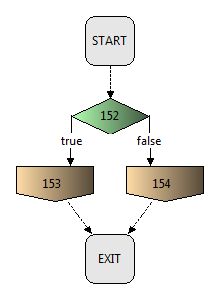
\includegraphics{isDecember.png}}
        \caption{Flow graph for method \texttt{isDecember(int)}.}
        \label{figure:december}
    \end{center}
\end{figure}

\begin{figure}[htpb!]
    \begin{center}
        \resizebox{3.89 cm}{!}{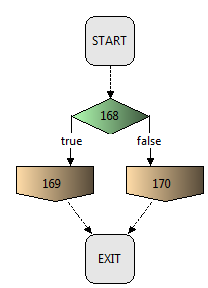
\includegraphics{isFebruary.png}}
        \caption{Flow graph for method \texttt{isFebruary(int)}.}
        \label{figure:february}
    \end{center}
\end{figure}

\begin{figure}[htpb!]
    \begin{center}
        \resizebox{5.55 cm}{!}{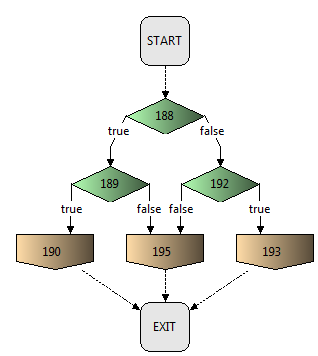
\includegraphics{isLeapYear.png}}
        \caption{Flow graph for method \texttt{isLeapYear(int)}.}
        \label{figure:leap-year}
    \end{center}
\end{figure}

\begin{figure}[htpb!]
    \begin{center}
        \resizebox{3.89 cm}{!}{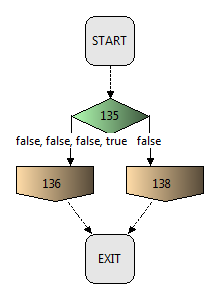
\includegraphics{isThirtyDayMonth.png}}
        \caption{Flow graph for method \texttt{isThirtyDayMonth(int)}.}
        \label{figure:thirty-day}
    \end{center}
\end{figure}

\begin{figure}[htpb!]
    \begin{center}
        \resizebox{4.62 cm}{!}{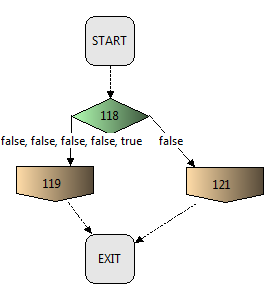
\includegraphics{isThirtyOneDayMonth.png}}
        \caption{Flow graph for method \texttt{isThirtyOneDayMonth(int)}.}
        \label{figure:thirty-one-day}
    \end{center}
\end{figure}

\begin{figure}[h!]
    \begin{center}
        \resizebox{13.6 cm}{!}{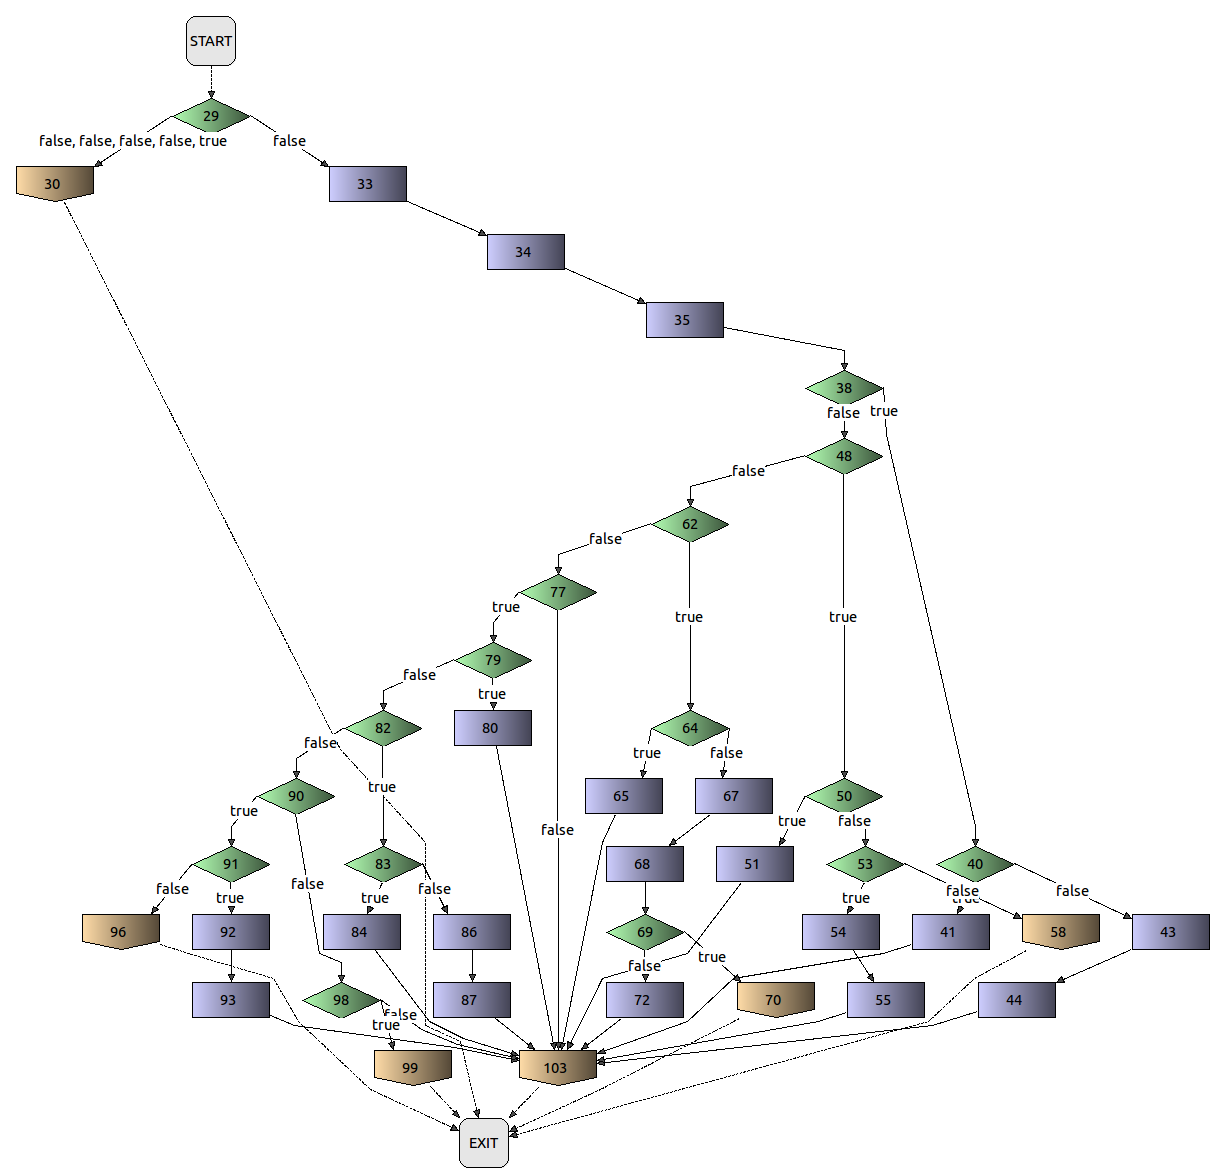
\includegraphics{run.png}}
        \caption{Flow graph for method \texttt{run(int, int, int)}.}
        \label{figure:run}
    \end{center}
\end{figure}

\section*{Assignment 5}

If we want to achieve a hundred percent coverage on both statements and decisions we can only focus on the decisions, also called branches. If we achieve 100\% branch coverage we will also get 100\% statement coverage. Conditions has to be taken independently to make sure that we cover them all.

\subsection*{isDecember}

The first method has only two branches and three statements. The condition is that either is it the twelfth month, or it's not. To get full coverage we only need one test case were we are at the twelfth month and one were it's not.

\begin{table}[h]
	\begin{tabular}{l}
		Test Case\\
		isDecember(10) $\rightarrow$ false\\
		isDecember(12) $\rightarrow$ true		
	\end{tabular}
\end{table}

\subsection*{isFebruary}

Next method is just like the previous one. The test cases will almost look the same.

\begin{table}[h]
	\begin{tabular}{l}
		Test Case\\
		isFebruary(1) $\rightarrow$ false\\
		isFebruary(2) $\rightarrow$ true		
	\end{tabular}
\end{table}

\subsection*{isLeapYear}

Third method is a bit more complicated then the previous one with a total number of 6 branches. Like was mentioned before, if we make sure that each branch is covered we have also fully covered all of the statements. Fortunately all of the decisions are again based upon a variable being equal, or not equal, to a certain value.

\begin{table}[h]
	\begin{tabular}{l}
		Test Case\\
		isLeapYear(500) $\rightarrow$ false\\
		isLeapYear(400) $\rightarrow$ true\\
		isLeapYear(24) $\rightarrow$ true\\
		isLeapYear(1999) $\rightarrow$ false		
	\end{tabular}
\end{table}

\subsection*{isThirtyDayMonth}

The method that checks if the current month has thirty days is a bit tricky. It might seem that we would have to produce test cases for each possible condition, but that's not entirely true. 

Since they are all compared between OR-operators, the first value to give \textbf{true} will satisfy the IF-statement. To cover all the decisions and the branches it will only be required to test all the values of a month that will result in a truth, as well as one test were \textbf{false} is returned.

\begin{table}[h]
	\begin{tabular}{l}
		Test Case\\
		isThirtyDayMonth(4) $\rightarrow$ true\\
		isThirtyDayMonth(6) $\rightarrow$ true\\
		isThirtyDayMonth(9) $\rightarrow$ true\\
		isThirtyDayMonth(11) $\rightarrow$ true\\		
		isThirtyDayMonth(12) $\rightarrow$ false\\
	\end{tabular}
\end{table}

\subsection*{isThirtyOneDayMonth}

Next method has the principle of its conditions as the previous one. A difference is that there are now 6 branches, instead of 5.

\begin{table}[h]
	\begin{tabular}{l}
		Test Case\\
		isThirtyOneDayMonth(1) $\rightarrow$ true\\
		isThirtyOneDayMonth(3) $\rightarrow$ true\\
		isThirtyOneDayMonth(5) $\rightarrow$ true\\
		isThirtyOneDayMonth(8) $\rightarrow$ true\\		
		isThirtyOneDayMonth(10) $\rightarrow$ true\\
		isThirtyOneDayMonth(11) $\rightarrow$ false\\
	\end{tabular}
\end{table}

\subsection*{run}

The last method is the most complicated one. Actually it is not a very good written method, for instance it has a cyclomatic complexity of twenty one and thirty six different branches. If we start with the leftmost branches at the top in figure \ref{figure:run} they are, like previous methods, together in one IF-statement with OR-operators.

\begin{table}[h]
	\begin{tabular}{l}
		Test Case\\
		run(0, *, *) $\rightarrow$ ``invalid Input Date''\\
		run(*, 0, *) $\rightarrow$ ``invalid Input Date''\\
		run(*, 13, *) $\rightarrow$ ``invalid Input Date''\\
		run(*, *, 1800) $\rightarrow$ ``invalid Input Date''\\		
		run(*, *, 2022) $\rightarrow$ ``invalid Input Date''\\
	\end{tabular}
\end{table}

The next set of test cases should now be created to take the right path instead. We will also have the opportunity to reuse the test cases for each of the private methods. If we consider the outer block of the next IF-statement the program performs checks on the current month. 

The test cases written last in this section will be the ones that are going to be implemented. This is because the method \texttt{run} is the only public method, which means the rest cannot be accessed from without the class, for example, from a test class.

If we want to have \textbf{true} returned we have to make sure to use the same cases as before. However, it is possible to combine the cases which returns \textbf{false} from one method with a case that return \textbf{true} for another method. 

\begin{table}[h]
	\begin{tabular}{l}
		Test Case\\
		run(*, 1, *)\\
		run(*, 2, *)\\
		run(*, 3, *)\\
		run(*, 4, *)\\
		run(*, 5, *)\\
		run(*, 6, *)\\
		run(*, 8, *)\\
		run(*, 9, *)\\
		run(*, 10, *)\\
		run(*, 11, *)\\
		run(*, 12, *)\\
	\end{tabular}
\end{table}

Next we can move forward with days. The next block of IF-statements performs checks if the day depending on the month.


\end{document}
